\section{Qualitätsmessung der dekomprimierten Daten}
Bei verlustbehafteten Kompressionen muss die Qualität des dekomprimierten Bildes sichergestellt werden. Im optimalen Fall ähneln die dekomprimierten Daten ihren Originalen, sodass für das menschliche Auge keine Artefakte sichtbar sind.\\
Im Verlauf der Arbeit wurden zwei Metriken verwendet: Die Standardabweichung und eine angepasste PSNR-HVS-M. Für die ersten Tests wurde nur die Standardabweichung gemessen. Es stellte sich heraus, dass die Standardabweichung nicht ausreicht: Sichtbare Artefakte, wie hochfrequente Schwingungen um die Originallinie fallen nicht ins Gewicht. Der absolute Fehler bleibt klein, für das menschliche Auge jedoch sind solche Artefakte störend (Ein Beispiel für die Artefakte ist in Abbildung \ref{resultate:loesung1:dct:randbehandlung:jvhartefakte} im Abschnitt \ref{resultate:loesung1:dct:randbeh+byte} zu finden). Wie die Standardabweichung berechnet wird, ist im Abschnitt \ref{testsetup:ablauf} beschrieben. Für weitere Tests wurde zusätzlich die PSNR-HVS-M Metrik berechnet. Die Metrik stammt aus der Bildverarbeitung. Das Ziel des Fehlermasses ist es, eine hohe Korrelation zwischen der Metrik und dem menschlichen Augenmass zu erreichen. Wie die PSNR-HVS-M Metrik angepasst und umgesetzt wurde, ist im Abschnitt \ref{testsetup:psnr} beschrieben.\\
Für die Messungen wurden spezielle Aufnahmen der Feldlinien gewählt. Wie die Aufnahmen ausgewählt wurden, ist im Abschnitt \ref{testsetup:auswahl_erhebung} beschrieben.\\
[\baselineskip]
Subsample\\
[\baselineskip]
%meh
Eine Grenze für die Genauigkeit ist nicht festzulegen. Auch wenn eine Grenze gefunden wird, kann diese sich in der Zeit verändern. Im Fall der Feldlinien ist die Internetverbindung der Flaschenhals. Es kann sein, dass in Zukunft mehr Präzision bei mehr Platzbedarf verlangt wird. Deshalb werden die Verfahren, wenn möglich, mit unterschiedlichen Qualitätsstufen getestet und verglichen.

\subsection{Auswahl und Erhebung der Testdaten}\label{testsetup:auswahl_erhebung}
Die Testdaten sollen zu einem alle Randfälle abdecken, als auch durchschnittliche Fälle enthalten. Aus diesem Grund wurden insgesamt zehn Datensätze ausgewählt: Vier Datensätze mit hoher Sonnenaktivität, zwei mit wenig und vier zufällig. Für die vier Datensätzen mit hoher Aktivität wurde in den Jahren 2014 und 2013 nach den grössten Solare Flares gesucht. Für die Datensätze mit wenig Aktivität wurde das Gegenteil gemacht, nach Zeiträumen mit möglichst kleinen Solar Flares gesucht.\\
Die Feldlinien werden aber nur alle sechs Stunden berechnet und Solar Flares sind sehr spontane Ereignisse. Auch eine grosse Flare kann während den sechs Stunden angefangen und wieder aufgehört haben. Für die grossen Solar Flares wurde deshalb beachtet, dass die Datensätze vor dem Ereignis verwendet wurden. Grosse Solar Flares entladen das Feld, vor dem Ereignis ist das Magnetfeld komplexer.\\
[\baselineskip]
Wie im Abschnitt \ref{konzept:ist-komprimierung} beschrieben, wird bereits eine einfache verlustbehaftete Kompression durchgeführt. Für die Testdaten wurde diese entfernt, was die rohe Datenmenge entsprechend anwachsen liess auf etwa 10 MiBytes pro Aufnahme.

\subsection{Berechnung der Standardabweichung}\label{testsetup:ablauf}
Die Linien sollten sich ähneln. Das ist der Fall, wenn die dekomprimierte Kurve entlang der Originalen verläuft und keine grosse Ausschläge beinhaltet. Grosse seltene Abweichungen können das Aussehen massgebend verändern. Neue Amplituden einführen etc. Ein Fall für die Standardabweichung. \\
Schwierigkeit liegt darin, von der Abtastrate die Standardabweichung zu berechnen.

\subsubsection{Allgemeiner Fall}
\begin{figure}[!htbp]
	\center
	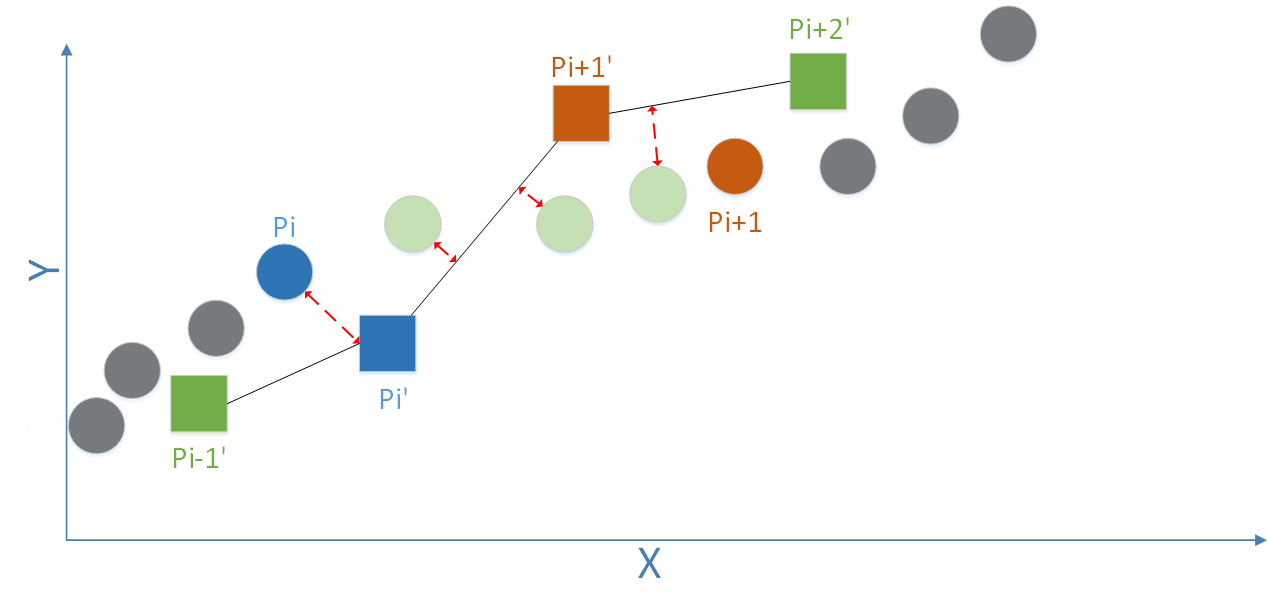
\includegraphics[width=0.8\textwidth,height=6cm,keepaspectratio]{./pictures/testsetup/errorcalc.png}
	\caption{Darstellung der Fehlerberechnung. Die Punkte sind die Originaldaten, die Quadrate sind die Punkte nach der Kompression.}
	\label{testsetup:ablauf:fehlerberechnung:diagramm}
\end{figure} 
Die Berechnung ist Dargestellt im Diagramm \ref{testsetup:ablauf:fehlerberechnung:diagramm}. Für jeden Punkt $p1'$ aus den dekomprimierten Punkten $D$, nehme $p1'$ und den folgenden Punkt und $P2'$. Ziehe eine Strecke $s$ durch $p1'$ und $p2'$. Suche von $p1'$ den Originalpunkt $P1$ aus allen Originalpunkten $O$ und rechne den Abstand aus zur Strecke $s$. Führe das für alle folgenden Originalpunkte durch, bis $p2$ erreicht wurde. Der Abstand $s$ zu $p2$ wird nicht mehr berechnet.\\
[\baselineskip]
\textbf{Abstandsberechnung eines Punktes zu einer Strecke}\\
Gegeben: Stecke $s$ mit Eckpunkten $A$ und $B$ und Punkt $P$.\\
Gesucht: Kürzeste Distanz zwischen $s$ und $P$\\
[\baselineskip]
Zuerst wird überprüft, ob eine Senkrechte durch $P$ überhaupt auf der Strecke $s$ zu liegen kommt. Das ist der Fall, wenn die Strecke $AP$ auf die Strecke $s$ projizierbar ist:
\begin{center}
$ t = \frac{\vec{AB}*\vec{AP}}{\lvert \vec{AB}\rvert ^2}$\\
  $0 \leq t \leq 1$
\end{center}
Wenn das nicht möglich ist, wird der kürzere Distanz von $P$ zu einem der Eckpunkte genommen. Falls aber eine Senkrechte auf $s$ zu liegen kommt, muss jetzt die Länge der Senkrechte berechnet werden. Aus der vorhgehenden Berechnung könnte man den Fusspunkt auf $s$ berechnen und dadurch die Distanz, oder man kann die Distanz direkt über das Kreuzprodukt berechnen.
\begin{center}
  $distance = \frac{\lvert \vec{BA}\times \vec{BP}\rvert}{\lvert \vec{BP} \rvert}$
\end{center}

\subsubsection{Randbehandlung}
\begin{figure}[!htbp]
	\center
	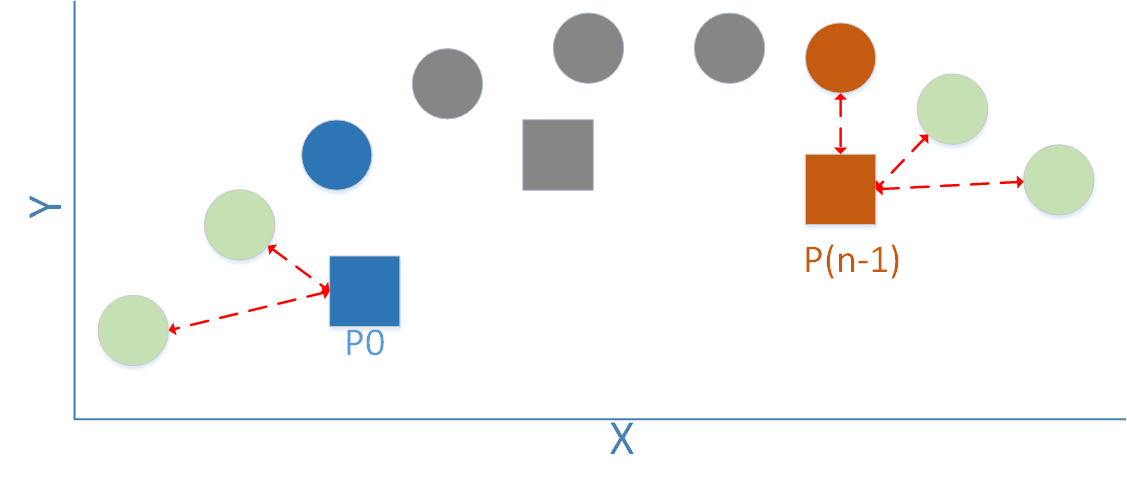
\includegraphics[width=0.8\textwidth,height=6cm,keepaspectratio]{./pictures/testsetup/randbehandlung.png}
	\caption{Darstellung der Fehlerberechnung. Die Punkte sind die Originaldaten, die Quadrate sind die Punkte nach der Kompression.}
	\label{testsetup:ablauf:randbehandlung:diagramm}
\end{figure}
Es ist möglich, dass die originalen Endpunkte durch eine Quantisierung verworfen wurden. Das bedeutet, wenn man den Fehler für den allgemeinen Fall berechnet, am Anfang und am Ende Originalpunkte existieren, für die nie eine Distanz berechnet wurde. Die Abbildung \ref{testsetup:ablauf:randbehandlung:diagramm} zeigt das Problem. Deshalb müssen die Abstände der Ränder von der Komprimierten- zur Original-Linie noch berechnet werden. Der Abstand vom ersten komprimierten Punkt (in der Abbildung P0) zu seinem Original wird schon im allgemeinen Fall berechnet.

\subsubsection{Berechnung der Standardabweichung}
\begin{center}
$\sigma(X) = \sqrt(variance(X))$\\
$variance(X) = \sum{(x_i - E(x_i))^2}$
\end{center}
Die Standardabweichung $\sigma$ einer Beobachtungsreihe $X$ $(x_1,x_2,x_3,\ldots, x_n-1)$ ergibt sich aus der Wurzel der Varianz von $X$. Die Varianz von $X$ kann errechnet werden, wenn man den Distanz jeder Beobachtung $x_i$ mit dem Erwartungswert $E(x_i)$ berechnet und quadriert. Die Beobachtung ist im diesen Fall ein Punkt der dekomprimierten Linie, während der Erwartungswert der Originalpunkt ist. Die Distanz wird mit dem besprochnen Verfahren \ref{testsetup:ablauf} berechnet. Die Summe der quadratischen Abstände ergibt die Varianz. Die Varianz wird über alle Testdaten berechnet, somit erhält man für einen Test genau eine Standardabweichung.

\subsection{Berechnung der angepassten PSNR-HVS-M}\label{testsetup:psnr}
Die PSNR (Peak-Signal-Noise-Ratio) Metrik ist ein weitverbreitetes Fehlermass in der Bildverarbeitung. Es kann für die Messung des Fehlers zwischen dekomprimierten Bild und dem Original eingesetzt werden. Das Problem der Metrik ist aber, dass es nicht immer mit der menschlichen Wahrnemung korreliert. Ponomarenko et al.  \cite{ponomarenko2007between:psnr} haben eine modifizierte PSNR entwickelt; die PSNR-HVS-M (Human Visual System Masking). In ihren Messungen erreichten sie eine hohe korrelation zwischen menschlicher Wahrnehmung von  verrauschten Bildern und dem neuen Fehlermass.\\
[\baselineskip]
$PSNR = 20 * log_(10)(MAX_I) - 10*log_(10)(MSE)$
$MSE = \frac{1}{n}\sum_{i=0}^{N-1}[E(i)-D(i)]^2$
PSNR setzt sich zusammen aus dem maximal möglichen Wert $MAX_I$ und dem ''Mean Squared Error´´ ($MSE$), der durchschnittliche Quadratische Fehler zwischen den Originaldaten $E()$ den dekomprimierten Daten $D()$.
Der Unterschied zwischen der PSNR und der PSNR-HVS-M liegt in der Berechnung des durchschnittlichen quadratischen Fehlers. Das Diagramm der Abbidlung \ref{testsetup:ablauf:psnr:flowchart} zeigt den Ablauf der neuen Berechnung.\\
\begin{figure}[!htbp]
	\center
	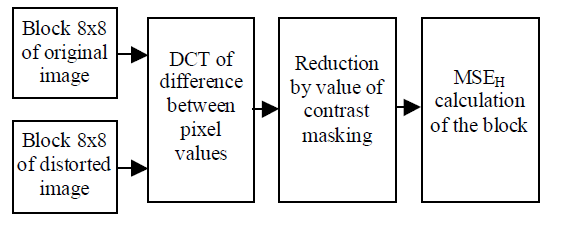
\includegraphics[width=0.8\textwidth,height=3.5cm,keepaspectratio]{./pictures/testsetup/psnr-hvs-m-flow.png}
	\caption{Flussdiagramm der PSNR-HVS-M Berechnung \cite{ponomarenko2007between:psnr}.}
	\label{testsetup:ablauf:psnr:flowchart}
\end{figure}
PSNR-HVS-M berechnet die Differenz zwischen dem Originalbild $E$ und dem verrauschtem Bild $D$ und führt die Daten mittels einer DCT in den Frequenzraum. Der nächste Schritt Contrast Maskin reduziert die Differenz, wenn das menschliche Auge den Frequenzunterschied nicht erkennen kann. Die Berechnung des $MSE_H$ Wertes erfolgt wieder gleich wie bei der PSNR.

\subsubsection{Contrast Masking}
Um das Contrast Masking zu berechnen, führt Ponomarenko et al. die gewichtete Energie der DCT Koeffizienten $E_w$ und den masking effect $E_m$ ein:\\
$E_w(X) = \sum_{i=0}^{7}\sum_{j=0}^{7}[X_{ij}]^2 C_{ij}$
$E_m(X) = \frac{1}{f_m}E_w(X)$
Wobei $X$ die Kosinus-Koeffizienten eines Blockes sind und $C$ die jeweiligen Gewichtungen zur Frequenz. Der Normalisierungsfaktor $f_m$ wurde experimentell ermittelt und auf $16$ festgelegt. Ponomarenko et al. argumentiert, dass der Unterschied zwischen einem Block $X_e$ und einem verrauschten Block $X_d$ unsichtbar sind, wenn:
$E_w(X_e-X_d) < max[E_m(X_e),E_m(X_d)]$
Diesen Sachverhalt wurde mit folgender Formel in der Fehlerberechnung miteinbezogen:

wobei $E_{norm} = \sqrt{max[E_m(X_e),E_m(X_d] / 64}$\\
[\baselineskip]
Wie gut die PSNR-HVS-M Metrik mit dem menschlichen Auge übereinstimmt, hängt vom Normalisierungsfaktor $f_m$ und von der Wahl der Gewichtungen $C$ ab. Ponomarenko et al. verwendeten die normalisierten und quadrierten Werte der JPEG Quantisierungsmatrix \cite{wallace1992jpeg}. Es ist zu beachten, dass der DC-Koeffizient nicht im Contrast Masking berücksichtigt wird, für den Wert wird die normale PSNR berechnet. Der DC-Koeffizient stellt die durchschnittliche Helligkeit in einem Block dar. Das menschliche Auge kann auch kleine Unterschiede in dieser Frequenz erkennen.

\subsubsection{Umsetzung und Anpassung für diese Arbeit}
Faktoren, Empirisch getestet mit algos. eher konservativ
maxvalue der psnr

\subsubsection{Wertebereich und Grenzen der PSNR}
Wann ist gut, wann knapp. Jetzt eher knapp
resultate mit $f_m$
16,40, 80